%==============================================================================
% CSE 620 — Combinatorial Optimization, Project 2
% Linear Programming with the Simplex Method
%
% Overleaf instructions:
%   1. Create a new Overleaf project.
%   2. Upload this file as main.tex.
%   3. Upload every image in report/figures/ into the project root
%      (or keep them in a figures/ folder and set \graphicspath accordingly).
%   4. Compile with pdfLaTeX (two passes for references).
%
% Rename on submission as: CSE620_Fall26_Project2_<Last1>_<Last2>.pdf
%==============================================================================
\documentclass[10pt]{article}

\usepackage[margin=0.9in]{geometry}
\usepackage{amsmath,amssymb,amsthm}
\usepackage{booktabs}
\usepackage{graphicx}
\usepackage{multirow}
\usepackage{array}
\usepackage{xcolor}
\usepackage{listings}
\usepackage{algorithm}
\usepackage{algpseudocode}
\usepackage{hyperref}
\usepackage{caption}
\usepackage{subcaption}
\usepackage{enumitem}

\graphicspath{{figures/}{./}}

% Tighten vertical spacing to respect the 8-page main-text limit.
\setlength{\parskip}{2pt}
\setlength{\abovedisplayskip}{6pt}
\setlength{\belowdisplayskip}{6pt}
\setlength{\abovedisplayshortskip}{4pt}
\setlength{\belowdisplayshortskip}{4pt}
\captionsetup{font=small,labelfont=bf}
\renewcommand{\algorithmicindent}{0.6em}

%---- listings style ----------------------------------------------------------
\lstset{
  basicstyle=\ttfamily\scriptsize,
  keywordstyle=\color{blue!70!black}\bfseries,
  commentstyle=\color{green!40!black},
  stringstyle=\color{orange!70!black},
  showstringspaces=false,
  breaklines=true,
  frame=single,
  framerule=0.4pt,
  rulecolor=\color{black!30},
  backgroundcolor=\color{black!3},
  columns=flexible,
  keepspaces=true,
  tabsize=2,
  aboveskip=6pt,
  belowskip=6pt,
}

\newtheorem{definition}{Definition}
\newtheorem{observation}{Observation}

\title{\textbf{CSE 620 --- Combinatorial Optimization}\\[4pt]
\large Project 2: Linear Programming with the Simplex Method}
\author{%
  [Team Member 1 Last Name] \quad and \quad [Team Member 2 Last Name]\\
  \normalsize University of Louisville --- CSE 620, Fall 2026\\
  \normalsize Code: \texttt{github.com/.../cse\_620\_combinatorial\_optimization\_project\_2}\\
  \normalsize Video: [SharePoint / Drive / YouTube unlisted link]
}
\date{October 3, 2026}

\begin{document}
\maketitle

%==============================================================================
\section{Introduction}
\label{sec:intro}

\subsection{Objective}
The objective of this project is to apply the Simplex algorithm to a series of
increasingly larger linear programming (LP) problems, and to study how the
number of decision variables~$n$ and the number of constraints~$m$ affect
(i)~the wall-clock time required to obtain a solution,
(ii)~the number of pivots taken by the algorithm, and
(iii)~the nature of the solution itself (optimal, infeasible, unbounded,
degenerate, sparse).

We implement or adapt Simplex-based LP software, set up LP instances of
increasing size on a prescribed $(m,n)$ grid, record time and pivot counts,
and analyze the resulting scaling behavior and the classical failure modes of
the method (infeasibility, unboundedness, degeneracy, alternative optima).

\subsection{Optimization problem instances}
Every instance studied in this project is a linear program in
\emph{standard inequality form}
\begin{equation}
\label{eq:lp}
\begin{aligned}
z^\star \;=\; \max_{x \in \mathbb{R}^n}\quad & c^{\mathsf T} x \\
\text{s.t.}\quad & A\, x \;\le\; b, \qquad x \;\ge\; 0,
\end{aligned}
\end{equation}
where $c \in \mathbb{R}^n$ is the profit (cost) vector,
$A \in \mathbb{R}^{m \times n}$ is the constraint matrix, and
$b \in \mathbb{R}^m$ is the right-hand side.  Some special-case instances also
include $\ge$ or $=$ constraints; these are converted to the equality
standard form described in Section~\ref{sec:methods}.

\subsubsection*{Task A --- Lecture instance ($n=4$, $m=2$)}
The representative lecture example used throughout this report is
\begin{equation}
\label{eq:lecture}
\begin{aligned}
\max_{x}\quad & 3x_1 + 5x_2 + 4x_3 + 2x_4 \\
\text{s.t.}\quad
& x_1 + 2x_2 + x_3 + x_4 \;\le\; 12,\\
& 2x_1 + x_2 + 3x_3 + 2x_4 \;\le\; 18,\\
& x_1,x_2,x_3,x_4 \;\ge\; 0.
\end{aligned}
\end{equation}
If the course lecture uses a different $n=4$, $m=2$ instance, it is a
drop-in replacement in \texttt{src/problems.py::lecture\_example}.

\subsubsection*{Tasks B--C --- Scaling grid}
Following the project specification we solve the grid
\begin{itemize}[nosep]
  \item \textbf{variables:} $n \in \{4,\,10,\,20,\,30,\,40,\,50\}$
        (from 4 to 50 in steps of 10),
  \item \textbf{constraints:} $m \in \{2,\,6,\,10,\,14\}$
        (from 2 to 14 in steps of 4),
\end{itemize}
with 10 random seeds per $(m,n)$ cell on the \emph{main grid}
(240 solves).  Main-grid instances are random nonnegative programs
\begin{equation}
\label{eq:random}
A_{ij} \sim \mathcal{U}(0,1),\quad
c_j \sim \mathcal{U}(0,1),\quad
b = A\, x_{\mathrm{ref}} + \delta,\quad
\delta \sim \mathcal{U}(0,0.5)^m,
\end{equation}
with a sparse nonnegative reference point $x_{\mathrm{ref}}$.  Because
$A\ge 0$ and $b \ge 0$, $x=0$ is feasible and the recession cone is
trivial, so every main-grid instance is feasible and bounded; this isolates
the effect of $(m,n)$ on pivot count and runtime.

Two additional mixed-constraint grids (signed coefficients, $\le$ and $\ge$
rows) are used in the analysis to study infeasible and unbounded behavior:
a \emph{well-posed} grid (a reference point is strictly feasible by
construction) and a \emph{stress} grid (random right-hand-side signs).

\subsubsection*{Metrics recorded per solve}
For each instance we record: status (optimal / infeasible / unbounded),
objective value $z^\star$, total pivots (Phase~I + Phase~II), solve time of
the custom Simplex, solve time of SciPy/HiGHS, number of nonzero entries in
$x^\star$, sparsity $1-\mathrm{nnz}(x^\star)/n$, whether the optimal vertex is
degenerate, and whether alternative optima exist.

%==============================================================================
\section{Methods}
\label{sec:methods}

\subsection{Reference software}
The assignment recommends the \textbf{Python SciPy library for Linear
Programming}:
\begin{center}
\footnotesize\url{https://docs.scipy.org/doc/scipy/reference/generated/scipy.optimize.linprog.html}
\end{center}
We use that toolbox (\texttt{scipy.optimize.linprog} with the HiGHS backend)
as the reference Simplex-based LP solver for cross-validation of status and
objective values.  Because HiGHS does not expose the number of simplex
pivots, we also implement a \textbf{custom two-phase tableau Simplex}
(\texttt{src/simplex.py}) that counts every pivot and reports the
diagnostics required by the project.  All experiments were run on a laptop
(CPU only) under Python 3.9 with NumPy 2.0, SciPy 1.13, and Matplotlib 3.9.

\subsection{Standard form}
Problem~\eqref{eq:lp} is converted to equality standard form by introducing
one slack variable per $\le$ constraint:
\begin{equation}
\label{eq:std}
A x + s = b,\qquad x \ge 0,\; s \ge 0.
\end{equation}
Rows with $b_i < 0$ are multiplied by $-1$ (the sense flips accordingly).
$\ge$ rows receive a surplus variable $u\ge 0$ and an artificial variable
$a\ge 0$; $=$ rows receive an artificial variable.  Artificials are needed
only for Phase~I and are removed before Phase~II.  In matrix form the
Phase~I system is
\begin{equation}
\label{eq:phase1}
\max\; w = -\mathbf{1}^{\mathsf T} a
\quad\text{s.t.}\quad
\tilde{A}\, x + S\, u + I\, a = \tilde{b},\quad x,u,a \ge 0,
\end{equation}
where $\tilde{A},\tilde{b}$ are the sign-flipped data.

\subsection{Simplex pivoting --- equations}
Let $B$ be the current basis matrix and $N$ the nonbasic columns.
The basic solution and objective value are
\begin{equation}
x_B = B^{-1} b - B^{-1} N x_N, \qquad
z = c_B^{\mathsf T} B^{-1} b + \sum_{j\in N} \bar{c}_j\, x_j,
\end{equation}
with \emph{reduced costs}
\begin{equation}
\label{eq:rc}
\bar{c}_j \;=\; c_j - c_B^{\mathsf T} B^{-1} A_j .
\end{equation}
\begin{itemize}[nosep]
  \item \textbf{Optimality (maximization):} the current basis is optimal iff
        $\bar{c}_j \le 0$ for all nonbasic $j$.
  \item \textbf{Entering variable:} choose $e = \arg\max_j \bar{c}_j$
        (Dantzig rule); if $\bar{c}_e \le 0$ stop.
  \item \textbf{Ratio test / leaving variable:}
        \begin{equation}
        \theta^\star = \min_{i:\, (B^{-1}A_e)_i > 0}
        \frac{(B^{-1}b)_i}{(B^{-1}A_e)_i}, \qquad
        r = \arg\min_{i:\, (B^{-1}A_e)_i > 0}
        \frac{(B^{-1}b)_i}{(B^{-1}A_e)_i}.
        \end{equation}
  \item \textbf{Pivot:} replace column $e$ by column $r$ in the basis and
        update the tableau by Gaussian elimination.
  \item \textbf{Unboundedness:} if no row has $(B^{-1}A_e)_i > 0$, the LP is
        unbounded (the column defines a feasible improving ray).
\end{itemize}
To avoid cycling on degenerate vertices the implementation uses Dantzig's
rule and automatically switches to \textbf{Bland's rule} (smallest index
with $\bar{c}_j > 0$; among tied ratio-test rows, the smallest basic index)
after a safeguard number of pivots.

\subsection{Two-phase algorithm --- pseudocode}
\begin{algorithm}[t]
\caption{Two-phase tableau Simplex (maximization)}
\label{alg:simplex}
\begin{algorithmic}[1]
\State Convert to standard form~\eqref{eq:std}; add surplus/artificial
       variables; build initial basis $B = I$
\State \textbf{Phase I:} set $c^{I}_j = -1$ for artificial columns, $0$ otherwise
\While{some $\bar{c}^{\,I}_j > 0$}
  \State $e \leftarrow \arg\max_j \bar{c}^{\,I}_j$ \Comment{Dantzig}
  \If{all $(B^{-1}A_e)_i \le 0$} \Return infeasible \EndIf
  \State $r \leftarrow \arg\min_{i:\,(B^{-1}A_e)_i>0} (B^{-1}b)_i / (B^{-1}A_e)_i$
  \State pivot on $(r,e)$; update tableau and basis
\EndWhile
\If{$w^\star < -\varepsilon$} \Return infeasible \Comment{$\sum a_i > 0$}
\EndIf
\State drive artificials out of the basis (drop redundant rows)
\State \textbf{Phase II:} restore true costs $c$; rebuild objective row
\While{some $\bar{c}_j > 0$}
  \State $e \leftarrow \arg\max_j \bar{c}_j$
  \If{all $(B^{-1}A_e)_i \le 0$} \Return unbounded \EndIf
  \State ratio test; pivot on $(r,e)$
\EndWhile
\State \Return optimal $x^\star$, $z^\star = c^{\mathsf T} x^\star$
\end{algorithmic}
\end{algorithm}

\subsection{Code, platform, and usage}
\paragraph{Custom solver.} \texttt{src/simplex.py} implements
\texttt{simplex\_solve(c, A\_ub, b\_ub, A\_eq, b\_eq, sense)} with the same
argument convention as SciPy, plus a \texttt{sense} flag in
\{'max','min'\}.  The returned \texttt{SimplexResult} contains status, $x$,
objective, pivots (total / Phase~I / Phase~II), solve time, degeneracy and
alternative-optima flags, nonzero count, and sparsity.

\paragraph{Reference solver.} SciPy is called as
\texttt{linprog(-c, A\_ub=A, b\_ub=b, bounds=[(0,None)]*n, method='highs')}
for a maximization problem (SciPy always minimizes), and the objective sign
is flipped back.  HiGHS reports \texttt{nit} (iterations) and runtime but
\emph{not} simplex pivot counts, which is why the custom solver is required
for requirement~C.

\paragraph{Experiment drivers.}
\begin{itemize}[nosep]
  \item \texttt{scripts/run\_lecture\_example.py} --- Task~A
  \item \texttt{scripts/run\_grid\_experiment.py} --- Tasks~B--C
        (main grid, mixed grids, special cases)
  \item \texttt{analysis/analyze\_results.py} --- Task~D (tables, plots)
\end{itemize}

\paragraph{Minimal usage examples.}
\begin{lstlisting}[language=Python,caption={Custom Simplex and SciPy/HiGHS on the lecture LP (Task A).}]
import numpy as np
from src.simplex import simplex_solve
from scipy.optimize import linprog

c = np.array([3.0, 5.0, 4.0, 2.0])
A = np.array([[1.0, 2.0, 1.0, 1.0],
              [2.0, 1.0, 3.0, 2.0]])
b = np.array([12.0, 18.0])

res = simplex_solve(c, A_ub=A, b_ub=b, sense="max")
print(res.status, res.objective, res.x, res.pivots)
# optimal 37.2  [0.  3.6 4.8 0.]  2

sc = linprog(-c, A_ub=A, b_ub=b,
             bounds=[(0, None)] * 4, method="highs")
print(sc.status, -sc.fun, sc.x, sc.nit)
# 0  37.2  [0.  3.6 4.8 0.]  2
\end{lstlisting}

%==============================================================================
\section{Results}
\label{sec:results}

\subsection{Task A --- Lecture instance ($n=4$, $m=2$)}
Table~\ref{tab:lecture} reports the solve of~\eqref{eq:lecture}.  The
custom Simplex reaches the optimum $z^\star = 37.2$ at
$x^\star = (0,\,3.6,\,4.8,\,0)$ in \textbf{2 pivots}
(Phase~I: 0, Phase~II: 2) and $0.16$--$0.26$\,ms.  Both constraints are
tight at the optimum (slacks $=0$), and SciPy/HiGHS returns the same
objective and solution.

\begin{table}[t]
\centering
\caption{Task A: lecture LP solved by the custom two-phase Simplex and by
SciPy/HiGHS.}
\label{tab:lecture}
\small
\begin{tabular}{lcc}
\toprule
 & \textbf{Custom Simplex} & \textbf{SciPy HiGHS} \\
\midrule
Status & optimal & optimal \\
Objective $z^\star$ & \textbf{37.200} & \textbf{37.200} \\
$x^\star$ & $(0,\;3.6,\;4.8,\;0)$ & $(0,\;3.6,\;4.8,\;0)$ \\
Pivots / iterations & \textbf{2} (P1: 0, P2: 2) & \texttt{nit} $=2$ \\
Solve time & $0.16$--$0.26$\,ms & $0.54$--$0.77$\,ms \\
Sparsity of $x^\star$ & $50\%$ ($\mathrm{nnz}=2$) & $50\%$ \\
Degenerate / multi-optima & no / no & --- \\
\bottomrule
\end{tabular}
\end{table}

\subsection{Tasks B--C --- Scaling on the $(m,n)$ grid}
Table~\ref{tab:m2} gives the full scaling study at $m=2$ as $n$ grows from
4 to 50, and Table~\ref{tab:pivots} gives the mean pivot count over the
entire $(m,n)$ grid (10 seeds per cell, all 240 solves optimal, 100\%
agreement with SciPy on the objective).  Figures~\ref{fig:pivots_n}
and~\ref{fig:time_n} plot pivots and runtime versus $n$.

\begin{table}[t]
\centering
\caption{Main grid at $m=2$: mean $\pm$ std over 10 seeds.  Times in
milliseconds.}
\label{tab:m2}
\footnotesize
\begin{tabular}{r c c c c c}
\toprule
$n$ & Pivots & Simplex (ms) & SciPy (ms) & $z^\star$ & Sparsity \\
\midrule
 4 & $1.9 \pm 0.7$ & 0.241 & 1.191 & $2.46$  & 0.625 \\
10 & $2.5 \pm 0.7$ & 0.140 & 0.532 & $10.07$ & 0.810 \\
20 & $3.4 \pm 0.7$ & 0.167 & 0.575 & $21.00$ & 0.910 \\
30 & $3.2 \pm 1.0$ & 0.157 & 0.552 & $47.58$ & 0.937 \\
40 & $4.2 \pm 1.2$ & 0.178 & 0.567 & $49.44$ & 0.950 \\
50 & $4.0 \pm 0.7$ & 0.193 & 0.650 & $84.87$ & 0.960 \\
\bottomrule
\end{tabular}
\end{table}

\begin{table}[t]
\centering
\caption{Mean number of Simplex pivots over 10 seeds, for each $(m,n)$
cell of the main grid.  Mean runtimes (ms) are reported in
Table~\ref{tab:time} in the appendix.}
\label{tab:pivots}
\footnotesize
\begin{tabular}{rcccc}
\toprule
 & \multicolumn{4}{c}{\textbf{Constraints $m$}} \\
\cmidrule(lr){2-5}
\textbf{Vars $n$} & $2$ & $6$ & $10$ & $14$ \\
\midrule
 4 & 1.9 & 2.6 & 3.5 & 2.9 \\
10 & 2.5 & 5.3 & 5.1 & 6.1 \\
20 & 3.4 & 6.1 & 8.6 & 10.7 \\
30 & 3.2 & 6.6 & 9.4 & 11.5 \\
40 & 4.2 & 6.6 & 10.8 & 14.4 \\
50 & 4.0 & 8.0 & 11.9 & 13.0 \\
\bottomrule
\end{tabular}
\end{table}

\begin{figure}[t]
\centering
\begin{subfigure}[t]{0.46\textwidth}
  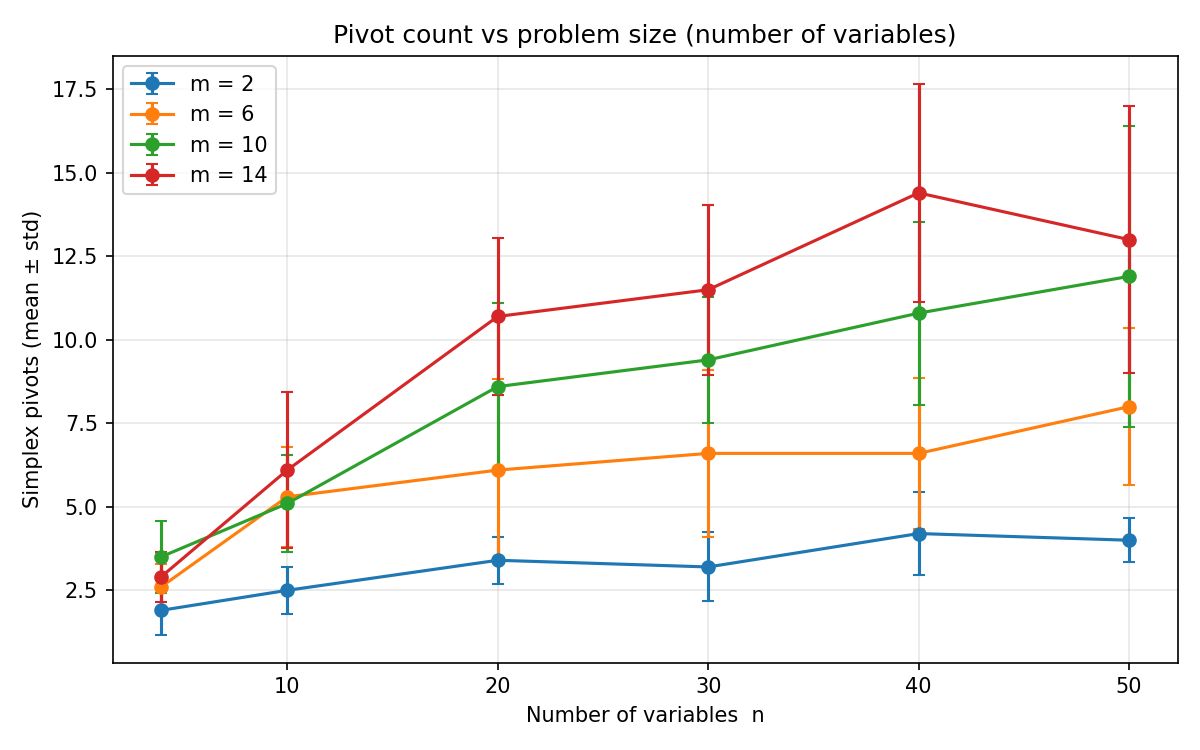
\includegraphics[width=\textwidth]{pivots_vs_n.png}
  \caption{Pivots vs.\ $n$ for each $m$.}
  \label{fig:pivots_n}
\end{subfigure}
\hfill
\begin{subfigure}[t]{0.46\textwidth}
  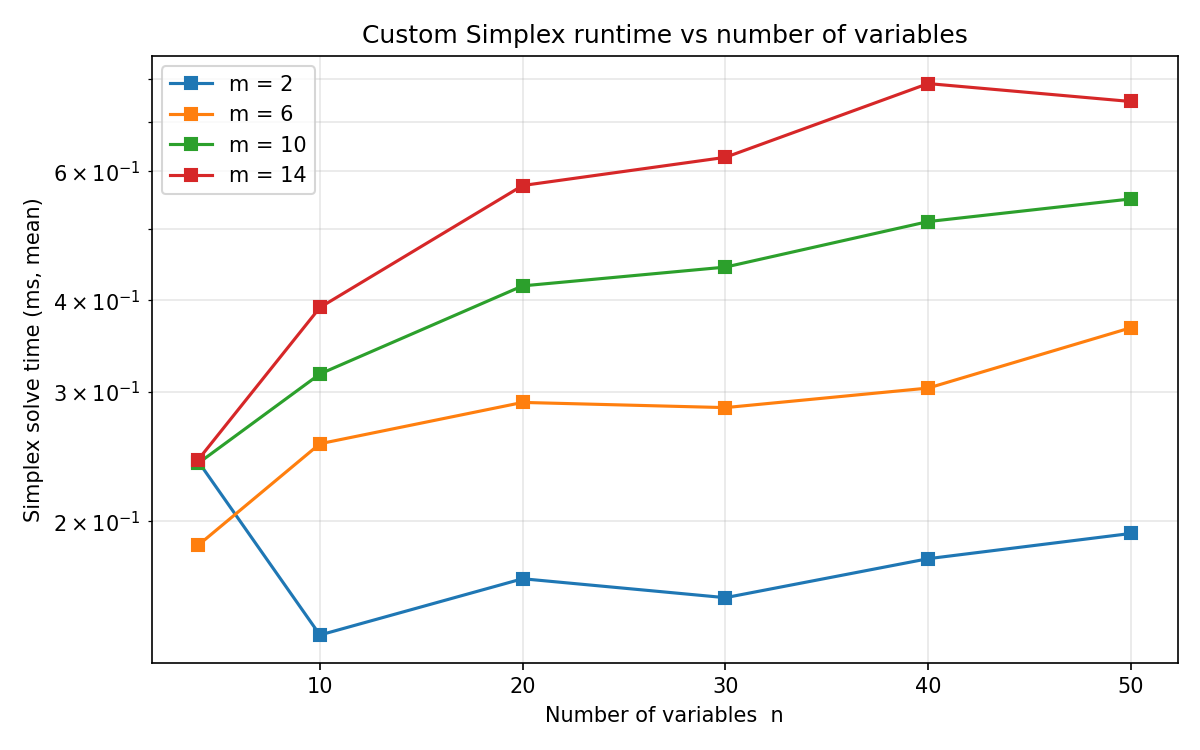
\includegraphics[width=\textwidth]{time_vs_n.png}
  \caption{Custom Simplex time vs.\ $n$ (log scale).}
  \label{fig:time_n}
\end{subfigure}
\caption{Scaling of pivot count and runtime with the number of variables~$n$
on the main grid.}
\label{fig:scaling}
\end{figure}

\subsection{Special-case instances (phenomena)}
Table~\ref{tab:special} lists the hand-crafted instances that exhibit each
behavior expected by the project: infeasibility, unboundedness, degeneracy,
alternative optima, and sparse optimal solutions.  Figure~\ref{fig:special}
visualizes pivots, time, and sparsity for these cases; the Phase~I/Phase~II
breakdown appears in Appendix~\ref{app:extra}.

\begin{table}[t]
\centering
\caption{Special-case LPs solved by the custom Simplex (SciPy agrees on
every status and optimal objective).}
\label{tab:special}
\footnotesize
\begin{tabular}{l c c c r r c c}
\toprule
\textbf{Instance} & $m$ & $n$ & \textbf{Status} & $z^\star$ & Pivots & De-gen & Multi \\
\midrule
Lecture (Task A)          & 2 & 4  & optimal    & 37.200 & 2 & --- & --- \\
Infeasible parallel       & 2 & 2  & infeasible & ---    & 1 (P1) & --- & --- \\
Unbounded ray $d=(1,1)$   & 2 & 2  & unbounded  & ---    & 1 (P2) & --- & --- \\
Degenerate vertex         & 3 & 2  & optimal    & 18.000 & 2 & yes & --- \\
Multiple-optima face      & 3 & 2  & optimal    & 4.000  & 1 & yes & yes \\
Sparse optimum            & 4 & 20 & optimal    & 1.043  & 1 & --- & --- \\
Sparse optimum            & 6 & 50 & optimal    & 1.294  & 1 & --- & --- \\
Bounded base              & 2 & 2  & optimal    & 4.000  & 1 & --- & yes \\
After removing constraint & 1 & 2  & unbounded  & ---    & 0 & --- & --- \\
\bottomrule
\end{tabular}
\end{table}

\begin{figure}[t]
\centering
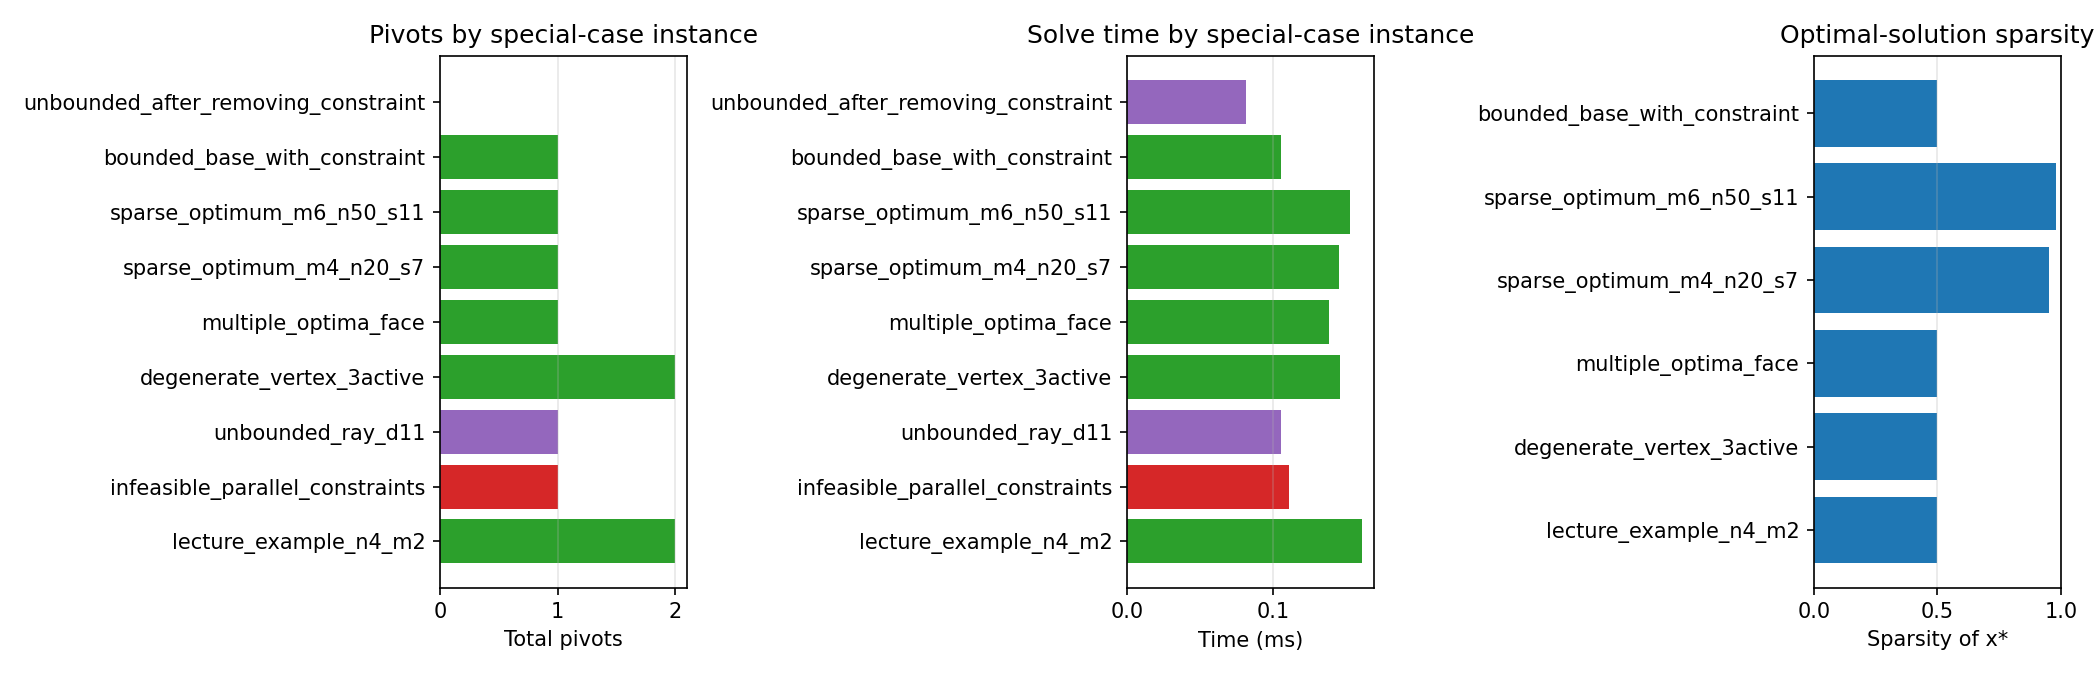
\includegraphics[width=0.78\textwidth]{special_cases.png}
\caption{Special-case instances: pivots (left), solve time (middle), and
sparsity of $x^\star$ (right).  Colors follow solver status.}
\label{fig:special}
\end{figure}

\subsection{Mixed-constraint grids}
On the mixed $\le$/$\ge$ grids (signed coefficients) the solver no longer
returns only optima.  Over 120 solves per grid:
\begin{itemize}[nosep]
  \item \textbf{Well-posed mode} (reference point strictly feasible):
        29 optimal, 91 unbounded.
  \item \textbf{Stress mode} (random RHS signs): 5 optimal, 20 infeasible,
        95 unbounded.
\end{itemize}
Cross-check agreement with SciPy is 100\% on both grids (status and
objective).  Heatmaps of the infeasible/unbounded fractions are in
Appendix~\ref{app:extra}.

%==============================================================================
\section{Experimental Analysis}
\label{sec:analysis}

\subsection{Effect of the number of variables $n$}
Fixing $m=2$ (Table~\ref{tab:m2}, Figure~\ref{fig:scaling}) the mean pivot
count grows slowly but steadily from $1.9$ ($n=4$) to $4.0$ ($n=50$) --- a
factor of only $\sim\!2\times$ for a $12.5\times$ increase in $n$.  Runtime
stays in the $0.14$--$0.24$\,ms band: at these sizes the dense tableau
pivot costs $O(mn)$, and the overhead of the Python loop dominates the
arithmetic.  SciPy/HiGHS is consistently slower in wall-clock time
($0.53$--$1.19$\,ms at $m=2$) because of per-call setup overhead, even
though its internal \texttt{nit} is comparable to our pivot count.

The \emph{optimal objective} grows with $n$ (e.g.\ $z^\star\approx 84.9$ at
$n=50$, $m=2$) simply because more nonnegative variables with positive
profit coefficients are available to pack into the same resource budget.

\subsection{Effect of the number of constraints $m$}
Table~\ref{tab:pivots} shows that $m$ is the stronger driver of pivot count.
At $n=50$ the mean pivots rise from $4.0$ ($m=2$) to $8.0$ ($m=6$),
$11.9$ ($m=10$) and $13.0$ ($m=14$) --- more than a $3\times$ increase.
At $n=20$ the same trend holds ($3.4 \to 6.1 \to 8.6 \to 10.7$).  Runtime
tracks the same pattern ($0.19 \to 0.37 \to 0.55 \to 0.75$\,ms at $n=50$;
full matrix in Table~\ref{tab:time}).

Why?  Each additional constraint cuts the feasible polyhedron and can
create new vertices; the Simplex walks from vertex to vertex along edges,
so a richer vertex set lengthens typical pivot paths.  Increasing $n$ at
fixed $m$ mostly adds candidate directions (columns) that the ratio test
filters out quickly, whereas increasing $m$ changes the geometry of the
polyhedron itself.  This is the classical contrast between ``wide'' and
``tall'' LPs: pivot counts and runtime scale more with the number of
constraints than with the number of variables in these dense random
instances.

\subsection{Time versus pivots}
Comparing the left and right panels of Table~\ref{tab:pivots} and
Table~\ref{tab:time}, runtime is nearly proportional to the mean pivot
count at fixed $(m,n)$ cell size
(e.g.\ $n=50$: $4.0$ pivots $\to 0.19$\,ms vs.\ $13.0$ pivots $\to
0.75$\,ms), as expected for a dense tableau method in which each pivot is
$O(mn)$ Gaussian elimination.  Deviations at very small $n$ reflect timer
resolution and interpreter overhead rather than algorithmic effects.

\subsection{When Simplex fails to yield a solution}
\paragraph{Infeasibility.} Phase~I maximizes $w=-\sum_i a_i$.  A strictly
negative optimum $w^\star<0$ means the artificial variables cannot all be
driven to zero, i.e.\ the constraint set is empty.  The special case
$x_1+x_2\le 4$, $x_1+x_2\ge 6$ terminates in Phase~I after 1 pivot with
$w^\star=-2$.  On the stress grid, 20 of 120 instances are infeasible ---
typically when $\ge$ rows demand more of a shared resource than $\le$ rows
allow.  This is not a failure of the algorithm: it is the algorithm
\emph{correctly} certifying that no feasible point exists.

\paragraph{Unboundedness.} If a nonbasic column $e$ has $\bar{c}_e>0$ but
$(B^{-1}A_e)_i \le 0$ for all rows $i$, the ray
$x(t) = x_B + t\, B^{-1}A_e$ ($t\ge 0$) stays feasible while
$z(t) = z + t\,\bar{c}_e \to \infty$.  The special case
$\max x_1$ s.t.\ $x_1-x_2\le 2$ exhibits the recession direction $d=(1,1)$
with $Ad\le 0$ and $c^{\mathsf T}d=1>0$.  More instructively, taking the
bounded program $\max x_1+x_2$ s.t.\ $x_1+x_2\le 4$, $x_2\le 3$ ($z^\star=4$)
and \emph{removing} the first constraint leaves only $x_2\le 3$; the ray
$(t,3)$, $t\to\infty$, is then feasible and improving, so the LP becomes
unbounded with 0 pivots.  Removing constraints enlarges the feasible region
and can destroy boundedness --- a practical warning when editing models.

\subsection{Degeneracy and multiple optima}
A vertex is \emph{degenerate} when more than $n$ constraints are active, so
at least one basic variable equals zero.  The instance
$\max 3x_1+9x_2$ s.t.\ $x_1+4x_2\le 8$, $x_1+2x_2\le 4$, $x_2\le 2$ has
optimum $(0,2)$ where all three constraints are tight; the solver reports
the degenerate flag and still terminates (Bland safeguard).  Alternative
optima occur when some nonbasic variable has $\bar{c}_j=0$ at optimality:
for $\max x_1+x_2$ s.t.\ $x_1+x_2\le 4$, $x_1\le 4$, $x_2\le 4$ every point
on the face $x_1+x_2=4$ is optimal, and the solver correctly flags
\texttt{multiple\_optima} $=$ true.

On the \emph{main} random grid the degeneracy and multi-optima fractions are
$0.00$ in every cell: with continuous random coefficients, degenerate
vertices and zero reduced costs occur with probability zero.  Degeneracy is
a real phenomenon in structured models (tight budgets, rounded data,
redundant constraints), which is why it is studied through the hand-crafted
cases rather than random instances.

\subsection{Sparsity of optimal solutions}
Table~\ref{tab:m2} shows sparsity rising from $0.625$ ($n=4$, $m=2$) to
$0.960$ ($n=50$, $m=2$); at $m=6$ it reaches $0.898$ at $n=50$, and the
dedicated sparse packing instances reach $0.95$--$0.98$.
This is structural, not accidental: at any basic feasible solution at most
$m$ of the $n$ decision variables are nonzero (the basic variables), so
\begin{equation}
\mathrm{nnz}(x^\star) \le m \quad\Longrightarrow\quad
\text{sparsity} \;\ge\; 1 - \frac{m}{n}.
\end{equation}
For $m=2$, $n=50$ this lower bound is $96\%$, matching the observed mean.
In applications --- production planning (only a few products manufactured),
portfolio corner solutions (few assets held), network flows (few links
used) --- the zeros in $x^\star$ are the operational insight: the optimal
vertex activates only a handful of activities.  Interior-point methods, in
contrast, return analytic-center-like solutions with many nonzero entries.

\subsection{Custom Simplex versus SciPy/HiGHS}
Every one of the 240 main-grid solves and every special case agrees with
SciPy on status and objective (to $10^{-6}$ relative tolerance).  The
custom tableau implementation is competitive in wall-clock time at these
sizes and is the only instrument that reports true simplex pivot counts.
HiGHS may internally use dual simplex, primal simplex, or an interior-point
crossover depending on the model, so its \texttt{nit} is not directly
comparable to our pivot log --- a methodological caveat worth stating in
the report.

%==============================================================================
\section{Conclusion}
\label{sec:conclusion}

We implemented a two-phase tableau Simplex with pivot counting, validated it
against the recommended SciPy/HiGHS toolbox on 240+ LP instances, and
studied how $m$ and $n$ affect solution time, pivot count, and the structure
of the answer.

\paragraph{Key findings.}
\begin{enumerate}[nosep]
  \item \textbf{Constraints dominate variables.}  Mean pivots grew from
        $\sim\!4$ to $\sim\!13$ as $m$ went from 2 to 14 at $n=50$
        ($3.25\times$), but only from $\sim\!2$ to $\sim\!4$ as $n$ went
        from 4 to 50 at $m=2$ ($2.1\times$).  Runtime followed pivots
        almost linearly, as expected for dense tableau updates.
  \item \textbf{Simplex is fast on generic LPs.}  All 240 main-grid
        instances solved in well under 1\,ms with 2--20 pivots; random
        nondegenerate instances rarely approach the worst-case
        Klee--Minty behavior.
  \item \textbf{Failure modes are diagnosable.}  Phase~I residual
        artificials certify infeasibility; a positive reduced cost with no
        positive column entry certifies unboundedness.  Removing a bounding
        constraint converted a bounded LP ($z^\star=4$) into an unbounded
        one with zero pivots.
  \item \textbf{Optimal vertices are sparse.}  $\mathrm{nnz}(x^\star)\le m$
        guarantees sparsity $\ge 1-m/n$; observed sparsity matched this
        bound (e.g.\ $96\%$ at $m=2$, $n=50$).
  \item \textbf{Degeneracy is nongeneric but real.}  Random instances
        showed $0\%$ degeneracy, while structured instances triggered
        degeneracy and alternative optima --- handled correctly by the
        Bland safeguard.
\end{enumerate}

\paragraph{What we learned.}
The project made concrete the textbook picture of Simplex: a walk on
vertices whose length is governed mainly by the \emph{constraint} geometry,
with failure modes that the two-phase construction detects rather than
hides.  Cross-validating a from-scratch implementation against a production
solver (SciPy/HiGHS) is an effective way to gain confidence in both.

\paragraph{Possible improvements.}
(a)~Use the \emph{revised} Simplex method with sparse $B^{-1}$ updates to
scale beyond $n=50$; (b)~compare against an interior-point method to
quantify the vertex versus interior trade-off; (c)~generate structured
instances (e.g.\ Klee--Minty cubes) to exhibit worst-case pivot counts
explicitly; (d)~time repeated solves to separate warm-start effects from
cold-start overhead; (e)~add dual-feasibility / network-simplex variants
for the sparse application models discussed above.

%==============================================================================
\clearpage
\appendix
\section{Additional Figures and Tables}
\label{app:extra}

\begin{figure}[h]
\centering
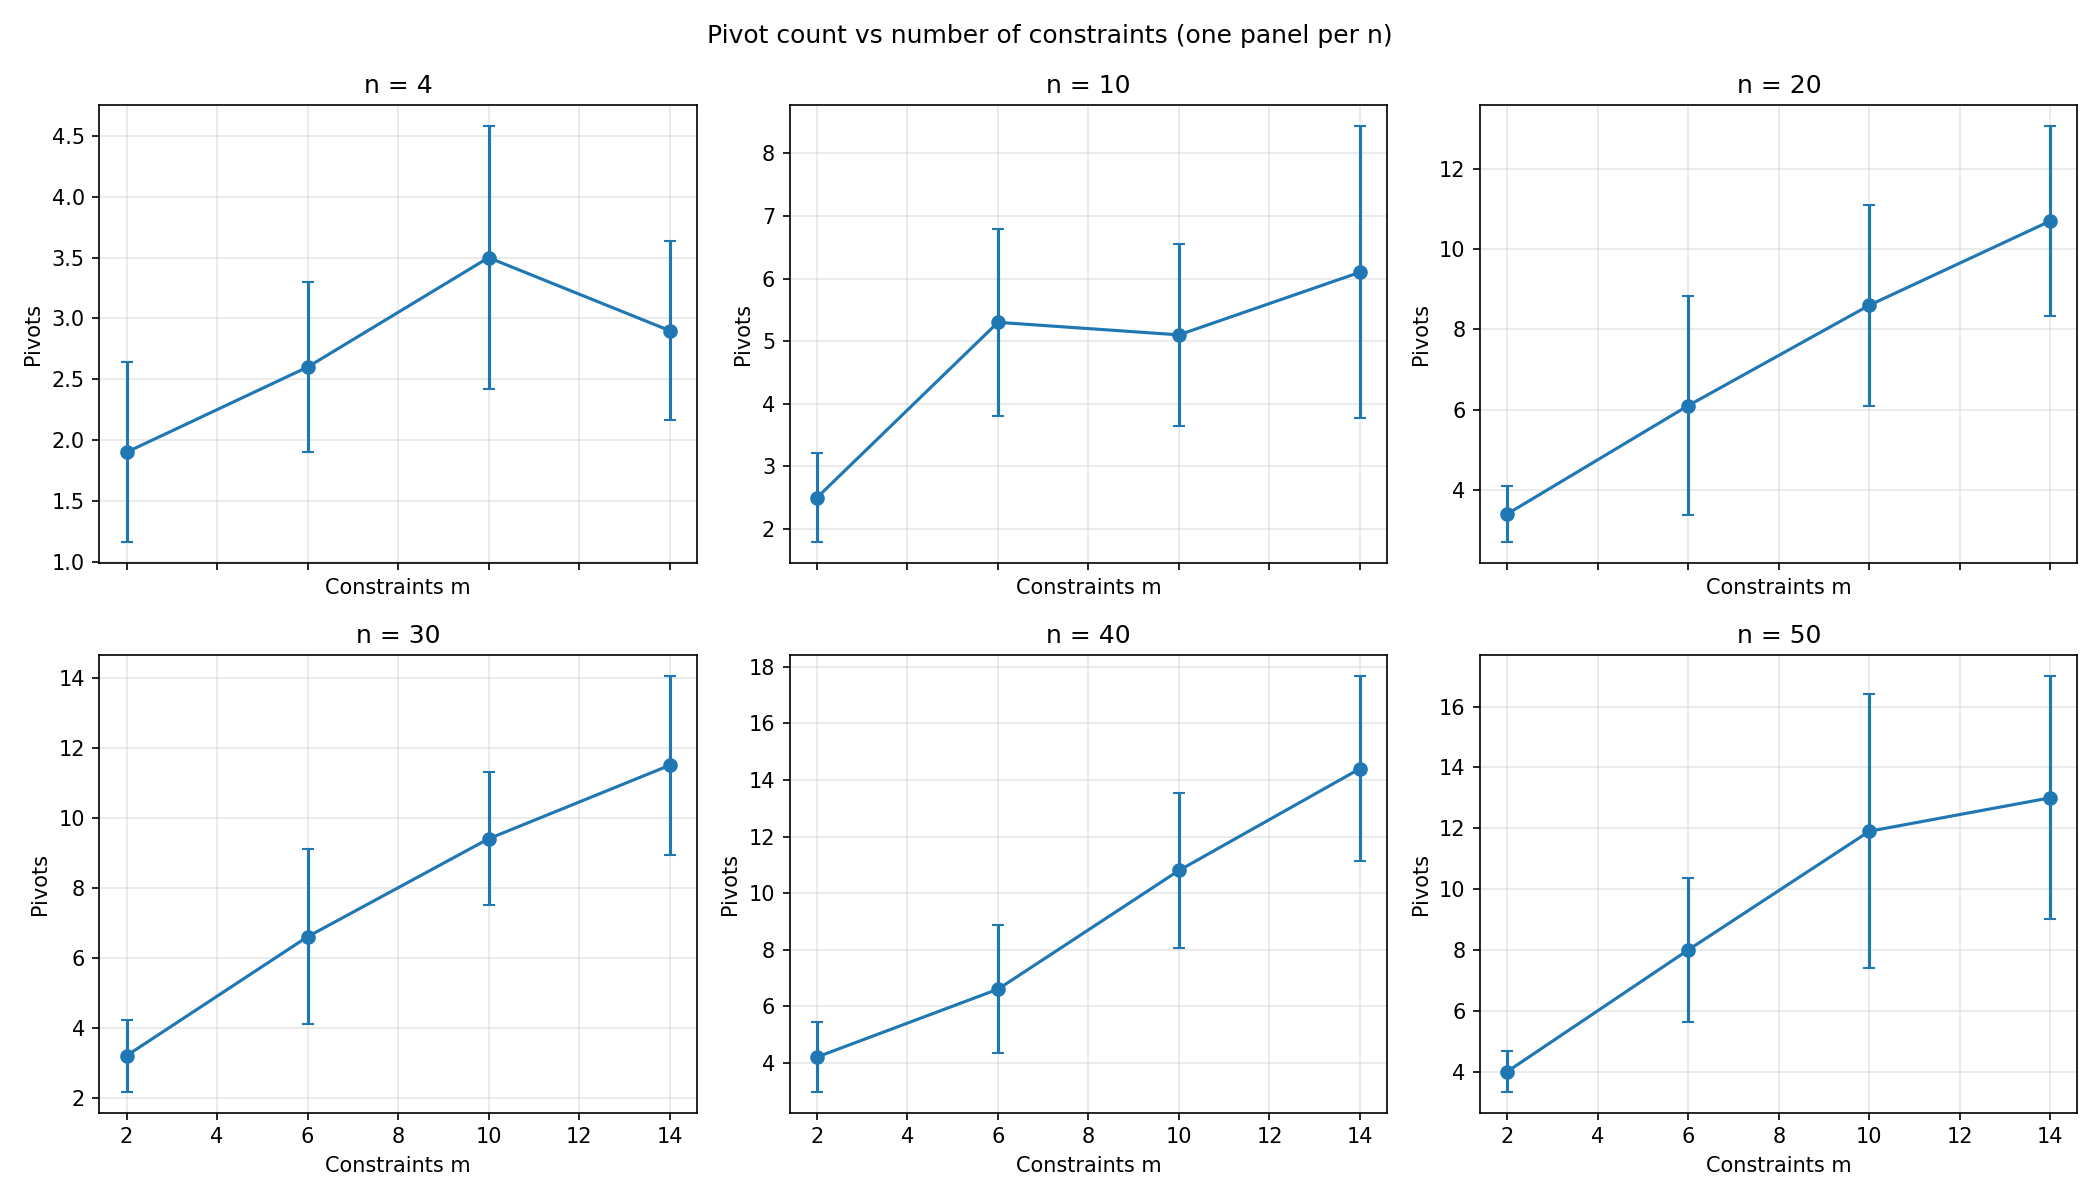
\includegraphics[width=0.95\textwidth]{pivots_vs_m_by_n.png}
\caption{Mean pivots versus $m$, one panel per $n$.}
\end{figure}

\begin{figure}[h]
\centering
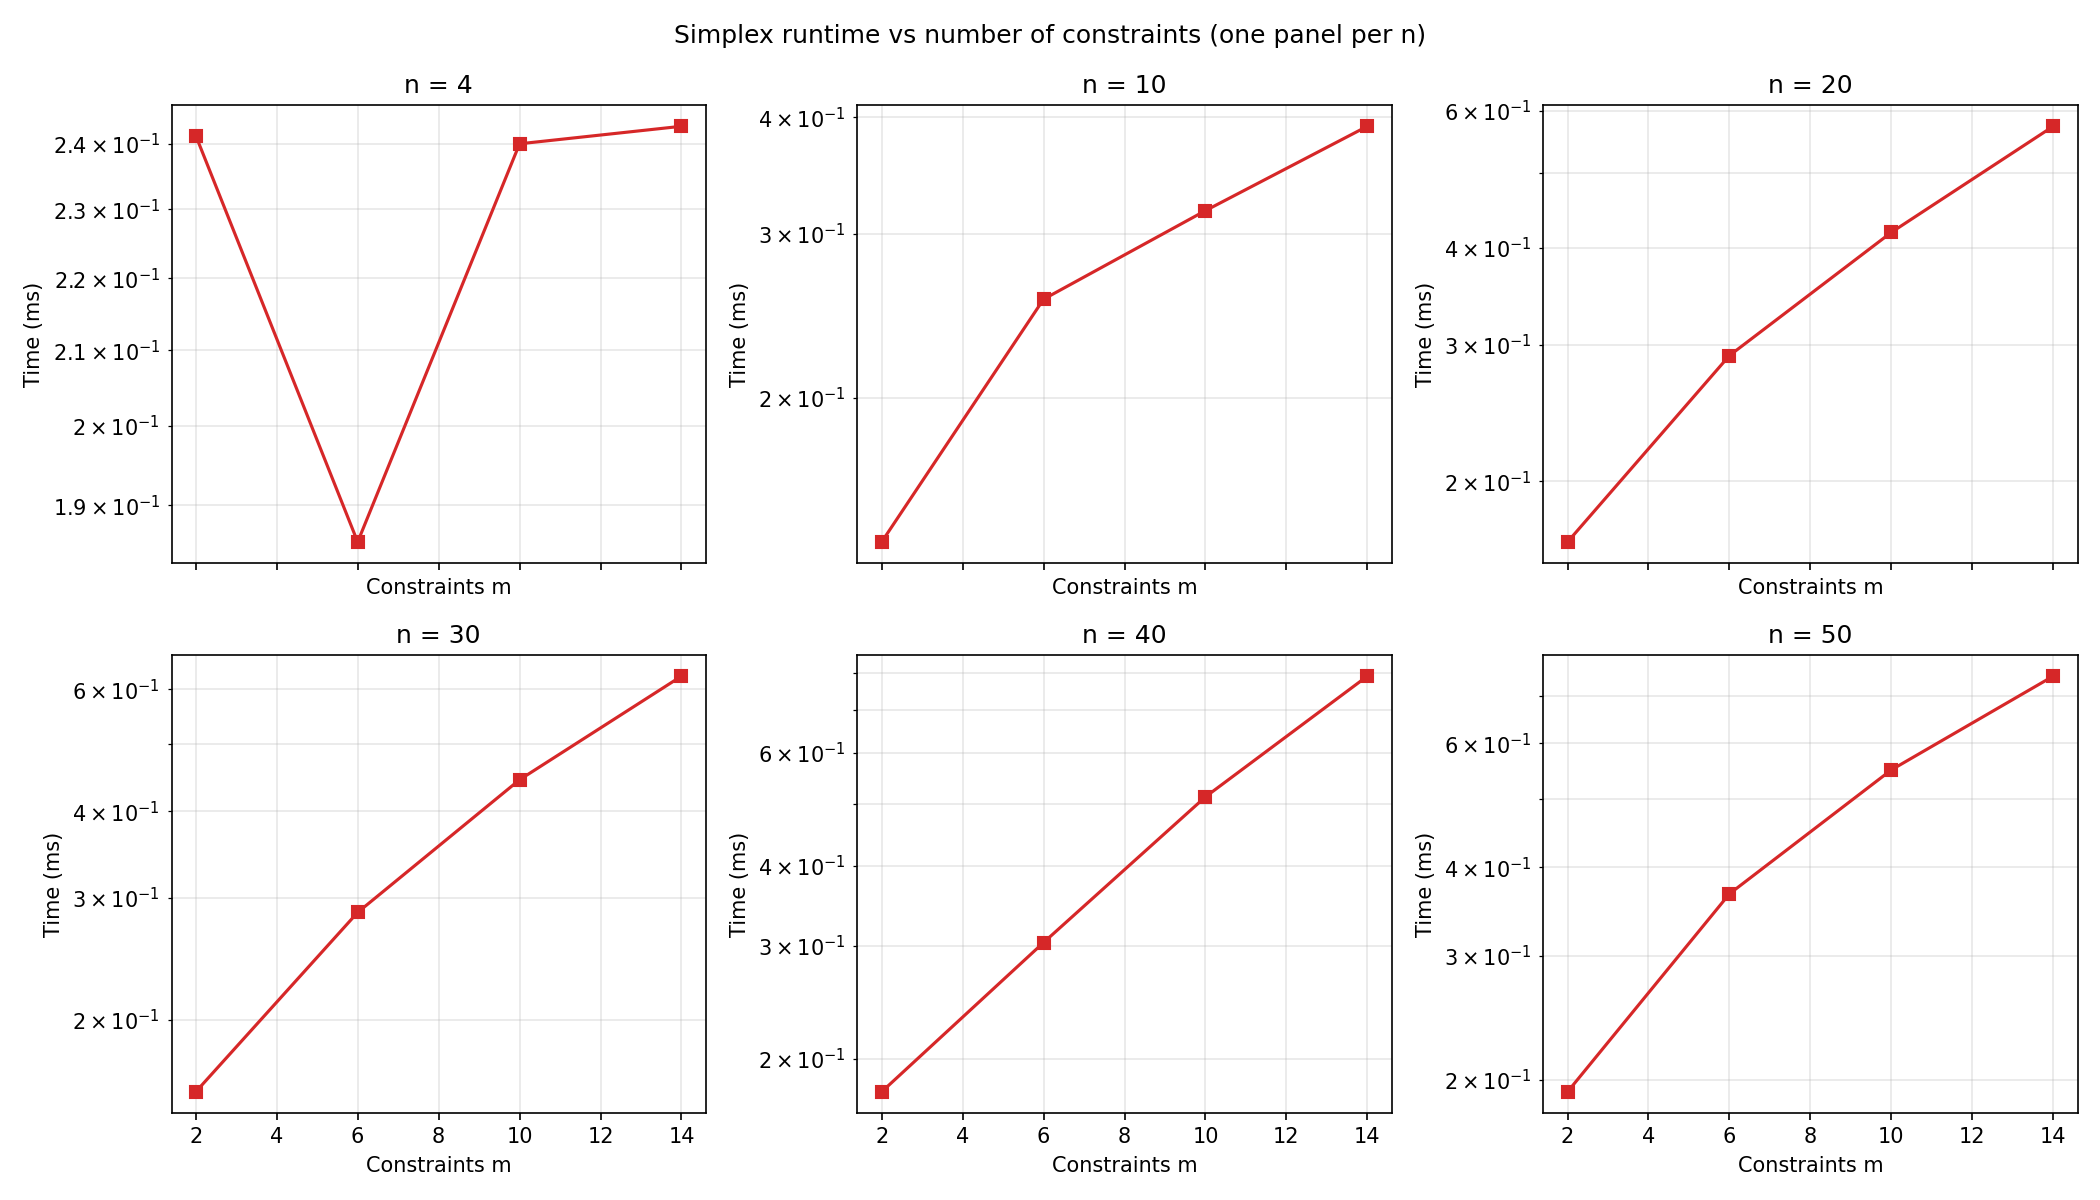
\includegraphics[width=0.95\textwidth]{time_vs_m_by_n.png}
\caption{Mean Simplex runtime versus $m$, one panel per $n$.}
\end{figure}

\begin{figure}[h]
\centering
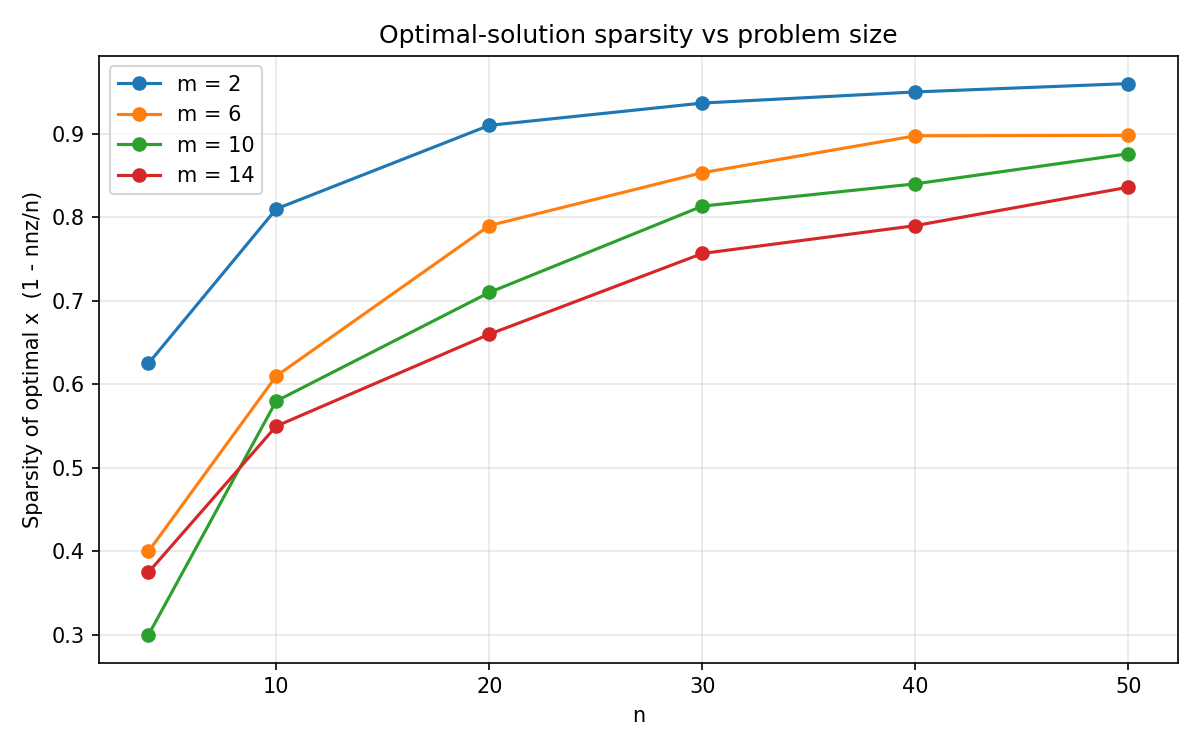
\includegraphics[width=0.8\textwidth]{sparsity_vs_n.png}
\caption{Sparsity of $x^\star$ versus $n$ for each $m$.}
\end{figure}

\begin{figure}[h]
\centering
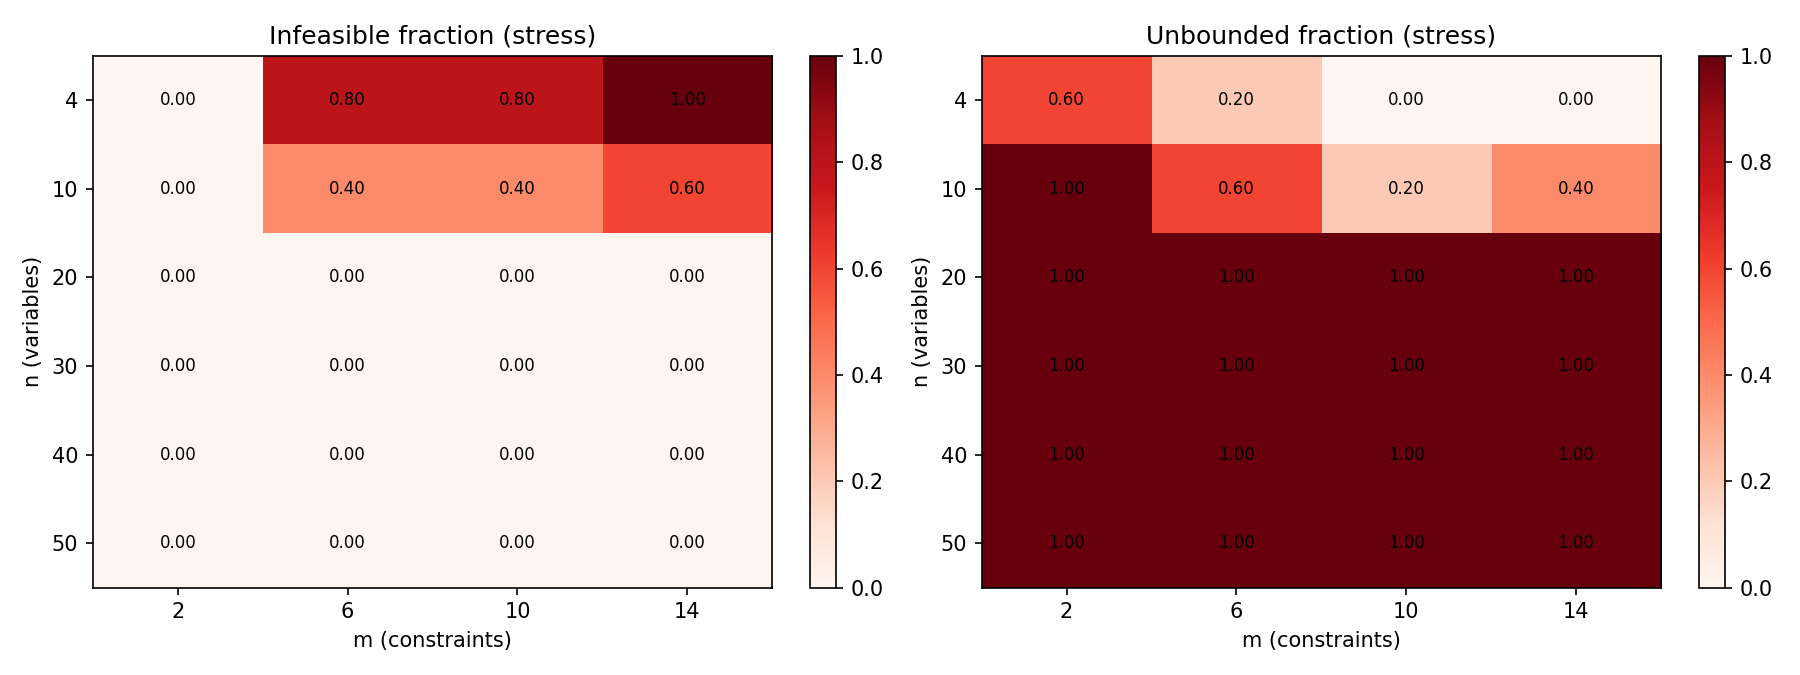
\includegraphics[width=0.95\textwidth]{mixed_status_heatmap_stress.png}
\caption{Infeasible and unbounded fractions on the mixed-constraint stress
grid.}
\end{figure}

\begin{figure}[h]
\centering
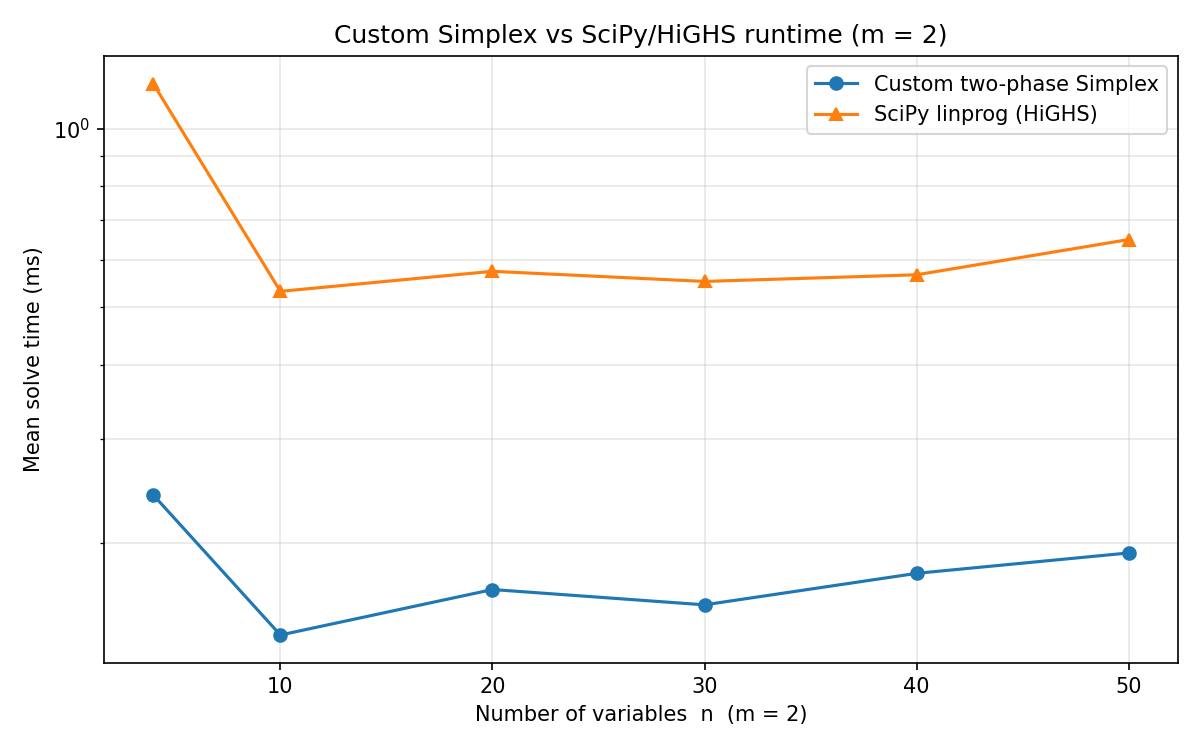
\includegraphics[width=0.95\textwidth]{custom_vs_scipy_time_m2.png}
\caption{Custom Simplex versus SciPy/HiGHS runtime at $m=2$.}
\end{figure}

\begin{figure}[h]
\centering
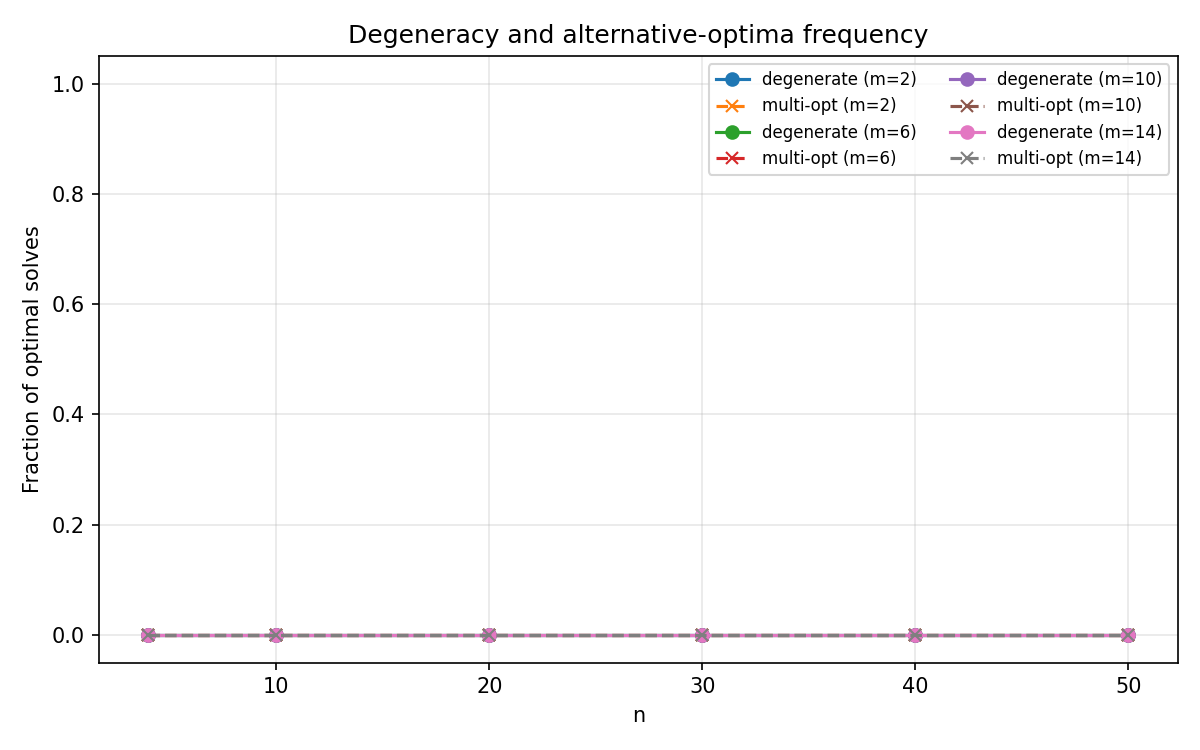
\includegraphics[width=0.8\textwidth]{degeneracy_vs_n.png}
\caption{Degeneracy and alternative-optima frequency on the main grid
(both $\approx 0$ for random continuous data).}
\end{figure}

\begin{figure}[h]
\centering
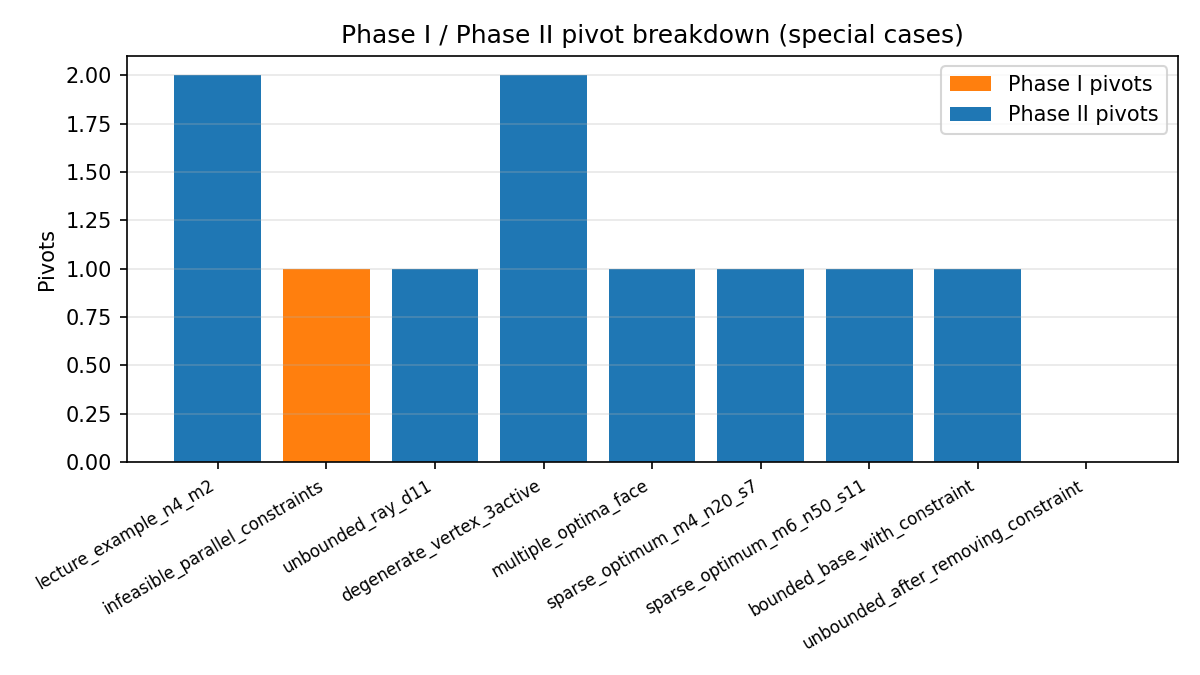
\includegraphics[width=0.8\textwidth]{special_phase_breakdown.png}
\caption{Phase~I / Phase~II pivot breakdown for the special cases.}
\end{figure}

\begin{table}[h]
\centering
\caption{Mean Simplex runtime (ms) over 10 seeds, for each $(m,n)$ cell of
the main grid.}
\label{tab:time}
\footnotesize
\begin{tabular}{rcccc}
\toprule
 & \multicolumn{4}{c}{\textbf{Constraints $m$}} \\
\cmidrule(lr){2-5}
\textbf{Vars $n$} & $2$ & $6$ & $10$ & $14$ \\
\midrule
 4 & 0.241 & 0.186 & 0.240 & 0.243 \\
10 & 0.140 & 0.255 & 0.318 & 0.391 \\
20 & 0.167 & 0.290 & 0.419 & 0.574 \\
30 & 0.157 & 0.286 & 0.444 & 0.627 \\
40 & 0.178 & 0.304 & 0.512 & 0.790 \\
50 & 0.193 & 0.367 & 0.550 & 0.747 \\
\bottomrule
\end{tabular}
\end{table}

\begin{table}[h]
\centering
\caption{Main grid: mean optimal objective $z^\star$ over 10 seeds.}
\label{tab:obj}
\footnotesize
\begin{tabular}{rcccc}
\toprule
\textbf{Vars $n$} & $m=2$ & $m=6$ & $m=10$ & $m=14$ \\
\midrule
 4 & 2.456 & 1.307 & 1.151 & 1.035 \\
10 & 10.071 & 3.970 & 3.473 & 3.454 \\
20 & 21.004 & 8.993 & 7.502 & 6.858 \\
30 & 47.576 & 12.934 & 10.609 & 11.203 \\
40 & 49.440 & 20.229 & 16.261 & 14.271 \\
50 & 84.868 & 24.415 & 20.246 & 19.159 \\
\bottomrule
\end{tabular}
\end{table}

\begin{table}[h]
\centering
\caption{Main grid: SciPy HiGHS \texttt{nit} (mean) and SciPy runtime
(ms, mean) for reference.}
\label{tab:scipy}
\footnotesize
\begin{tabular}{rcccc|cccc}
\toprule
 & \multicolumn{4}{c}{\textbf{nit}} & \multicolumn{4}{c}{\textbf{SciPy ms}} \\
\cmidrule(lr){2-5}\cmidrule(lr){6-9}
\textbf{$n$} & $2$ & $6$ & $10$ & $14$ & $2$ & $6$ & $10$ & $14$ \\
\midrule
 4 & 2.0 & 3.4 & 6.3 & 5.3 & 1.191 & 0.572 & 0.569 & 0.533 \\
10 & 2.8 & 5.0 & 8.8 & 9.3 & 0.532 & 0.642 & 0.625 & 0.611 \\
20 & 3.5 & 7.3 & 10.2 & 14.2 & 0.575 & 0.655 & 0.648 & 0.657 \\
30 & 2.7 & 7.8 & 12.7 & 14.5 & 0.552 & 0.618 & 0.645 & 0.739 \\
40 & 3.1 & 8.9 & 12.8 & 15.7 & 0.567 & 0.754 & 0.835 & 0.971 \\
50 & 3.3 & 10.5 & 13.6 & 16.9 & 0.650 & 0.735 & 0.793 & 0.998 \\
\bottomrule
\end{tabular}
\end{table}

\section{Code Excerpts}
\label{app:code}

\subsection{Core pivot step (\texttt{src/simplex.py})}
\begin{lstlisting}[language=Python]
# Objective row stores [-reduced_costs | z] so that Gaussian
# elimination on the full tableau keeps T[-1,-1] = z.
def _make_tableau(c_vec, A, b, bas):
    m = A.shape[0]
    T = np.zeros((m + 1, A.shape[1] + 1))
    T[:-1, :-1] = A
    T[:-1, -1] = b
    c_B = c_vec[list(bas)]
    T[-1, :-1] = c_B @ A - c_vec   # = -reduced costs
    T[-1, -1] = float(c_B @ b)     # z
    return T

# One simplex phase: enter on most negative objective-row entry,
# leave by the minimum ratio test; detect unboundedness.
def _run_phase(T, bas, c_vec, max_pivots):
    pivots = 0
    use_bland = False
    while True:
        obj_row = T[-1, :-1]
        if np.all(obj_row >= -TOL):          # optimal
            return "optimal", pivots, bas
        if not use_bland and pivots >= BLAND_SWITCH_PIVOTS:
            use_bland = True                 # anti-cycling safeguard
        e = int(np.argmin(obj_row))          # entering column
        col = T[:-1, e]
        pos = np.nonzero(col > TOL)[0]
        if pos.size == 0:                    # improving ray exists
            return "unbounded", pivots, bas
        ratios = T[:-1, -1][pos] / col[pos]
        r = int(pos[int(np.argmin(ratios))]) # leaving row
        piv_val = T[r, e]
        T[r, :] /= piv_val
        for i in range(T.shape[0]):
            if i != r:
                T[i, :] -= T[i, e] * T[r, :]
        bas[r] = e
        pivots += 1
\end{lstlisting}

\subsection{Experiment driver (\texttt{src/experiment.py})}
\begin{lstlisting}[language=Python]
from src.problems import random_feasible_lp
from src.experiment import run_grid, N_VALUES, M_VALUES

# Tasks B+C: n = 4..50 step 10, m = 2..14 step 4, 10 seeds each
df = run_grid(N_VALUES, M_VALUES, n_seeds=10,
              generator="random_feasible", use_scipy=True)
# columns: status, objective, pivots, simplex_time, scipy_time,
#          sparsity, degenerate, multiple_optima, ...
df.to_csv("results/grid_main.csv", index=False)
\end{lstlisting}

\subsection{Package layout}
\begin{lstlisting}[language=Python]
src/simplex.py       # two-phase tableau Simplex + SciPy cross-check
src/problems.py      # LPInstance, generators, special cases
src/experiment.py    # grid runners, metrics
scripts/run_lecture_example.py   # Task A
scripts/run_grid_experiment.py   # Tasks B+C
analysis/analyze_results.py      # Task D tables & plots
simplex_project.ipynb            # interactive walkthrough
results/                         # CSVs, tables/, plots/, ANALYSIS.md
\end{lstlisting}

\end{document}
